\documentclass[border=5pt]{standalone}
\usepackage{tikz}

\begin{document}
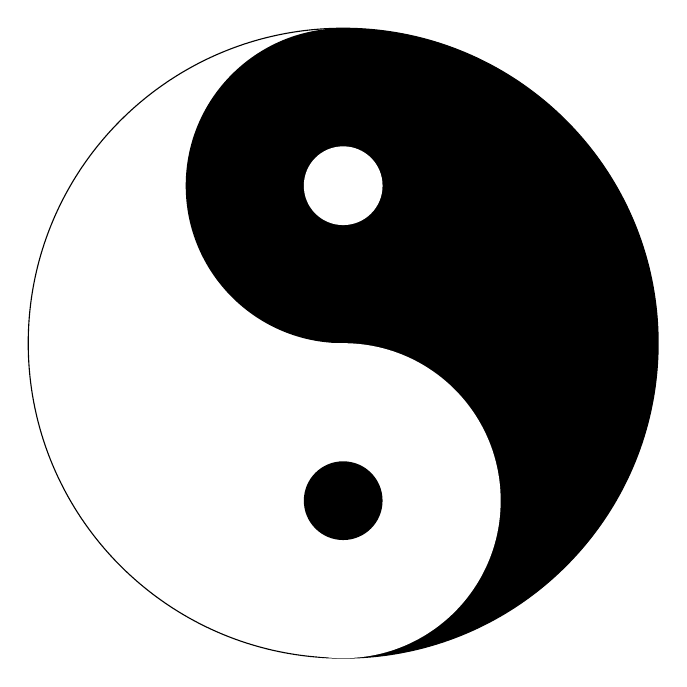
\begin{tikzpicture}
  
\draw(0,0) circle(4cm);  %画一个4cm的圆圈
%把圆的右半边填黑
\begin{scope}
  \clip(0,0) circle(4cm);
  \fill[black] (0,-4) rectangle (4,4);
\end{scope}

%填黑八卦图左边的半圆
\begin{scope}
  \clip(0,2) circle(2cm);
  \fill[black] (-4,0) rectangle (4,4);
\end{scope}

%填白八卦图右边的半圆
\fill[white] (0,-2) circle(2cm);

%把黑色部分的小圆圈填为白色
\fill[white] (0,2) circle(0.5cm);

% %绘制下面的白色圆圈
\fill(0,-2) circle(0.5cm);

\end{tikzpicture}

\end{document}